\section{Summary}
\label{chap:correctness:summary}

% \todo{Add a conceptual model (reuse from JSS): Add in summary?
% Consistency relation (fine-grained induces model level one)
% Consistency preservation rule (preserved relation (either model-level or fine-grained)
% Transformation (combined consistency relations and consistency preservation rule)
% Orchestration function (orchestrates transformations)
% Application function (applies transformations according to orchestration)
% }

\begin{figure}
    \centering
    %\newcommand{\hdistance}{17em}
\newcommand{\vdistance}{6.2em}

\begin{tikzpicture}[
    model style/.style={color=darkgray},
    concept/.style={draw, minimum width=8.5em, minimum height=3em, inner sep=0.5em},
    model concept/.style={model style, concept},
    metamodel concept/.style={concept, align=center},
    model relation/.style={model style},
    metamodel relation/.style={},
]

%\node[model concept, minimum height=1.5em, minimum width=6em] (model) {Model};
%\node[metamodel concept, minimum height=1.5em, minimum width=6em, right=0.7*\hdistance of model.north, anchor=north] (metamodel) {Metamodel};

\node[metamodel concept, minimum height=1.5em] (metamodel) {Metamodel};

\node[metamodel concept, below left=0.9*\vdistance and 0.5*\hdistance of metamodel.north, anchor=north] (mlcr) {Model-Level\\ Consistency Relation};
\node[metamodel concept, below right=0.9*\vdistance and 0.5*\hdistance of metamodel.north, anchor=north] (cr) {(Fine-Grained)\\ Consistency Relation};
\node[metamodel concept, below=1.15*\vdistance of mlcr.north, anchor=north] (cpr) {Consistency\\ Preservation Rule};
\node[metamodel concept, below=1.15*\vdistance of cr.north, anchor=north] (transformation) {Transformation};
\node[metamodel concept, below=\vdistance of transformation.north, anchor=north] (orchestration) {Orchestration\\ Function};
\node[metamodel concept, below=\vdistance of orchestration.north, anchor=north] (network) {Transformation\\ Network};
\node[metamodel concept, left=\hdistance of orchestration.north, anchor=north] (application) {Application\\ Function};

%\draw[model relation, dashed, -angle 60] (model) -- node[uml cardinality start, pos=0, below right] {*} node[uml association name, above] {\guillemotleft instance of\guillemotright} node[uml cardinality end, pos=1, below left] {1} (metamodel);

\draw[metamodel relation, open diamond-angle 60] (mlcr) -- node[uml cardinality start, pos=0, above right=0em and 1em] {*} node[uml association name, pos=0.35, above left=0em and -0.3em, align=center] {describes\\ consistency\\ between} node[uml cardinality end, pos=1, below right] {2} ([xshift=-1.5em]metamodel.south);
\draw[metamodel relation, open diamond-angle 60] (cr) -- node[uml cardinality start, pos=0, above left=0em and 1em] {*} node[uml association name, pos=0.35, above right=0em and -0.3em, align=center] {describes\\ consistency\\ between} node[uml cardinality end, pos=1, below left] {2} ([xshift=1.5em]metamodel.south);
\draw[metamodel relation, -angle 60] (cr) -- node[uml cardinality start, pos=0, below left] {*} node[uml association name, above, align=center] {implies} node[uml cardinality end, pos=1, below right] {1} (mlcr);

\coordinate (crosspoint) at ($(cpr)!0.5!(cr)$);
\draw[metamodel relation, -angle 60] (crosspoint) -- node[uml role start, pos=0, above=0.5em] {either or} node[uml cardinality end, pos=1, below left] {1} (mlcr);
\draw[metamodel relation, -angle 60] (crosspoint) -- node[uml cardinality end, pos=1, below right] {1..*} (cr);
\draw[metamodel relation, dashed] ([xshift=-2em]crosspoint) -- ([xshift=2em]crosspoint);
\draw[metamodel relation, -angle 60] ([yshift=0.3em]cpr.east) -| node[uml cardinality start, pos=0, above right=0em] {*} node[uml association name, pos=1, below left, align=center] {preserves\\ consistency\\ to} ([xshift=-0.5em]crosspoint);
\draw[metamodel relation, -angle 60] ([yshift=0.3em]transformation.west) -| node[uml cardinality start, pos=0, above left] {*} node[uml association name, pos=1, below right, align=center] {consists\\ of} ([xshift=0.5em]crosspoint);
\draw[metamodel relation, open diamond-angle 60] ([yshift=-0.5em]transformation.west) -- node[uml cardinality start, pos=0, below left] {*} node[uml association name, pos=0.5, below, align=center] {consists of} node[uml cardinality end, pos=1, below right] {1} ([yshift=-0.5em]cpr.east);

\draw[metamodel relation, -angle 60] (orchestration) -- node[uml cardinality start, pos=0, above left] {*} node[uml association name, right] {orchestrates} node[uml cardinality end, pos=1, below left] {*} (transformation);
\draw[metamodel relation, -angle 60] (application) -- node[uml cardinality start, pos=0, above left] {*} node[uml association name, above, pos=0.35, sloped] (executes_label) {executes} node[uml cardinality end, pos=1, below right] {*} (transformation);
\draw[metamodel relation, densely dashed] (executes_label) -- node[uml association name, below, sloped] {orchestrated by} node[uml cardinality end, pos=1, above left=0.5em and 0em] {1} (orchestration.west);

\draw[metamodel relation, open diamond-angle 60] (network) -- node[uml cardinality start, pos=0, above left] {*} node[uml association name, right] {consists of} node[uml cardinality end, pos=1, below left] {1} (orchestration);
\draw[metamodel relation, open diamond-angle 60] (network.west) -- node[uml cardinality start, pos=0, above left] {*} node[uml association name, above, sloped] {consists of} node[uml cardinality end, pos=1, below left] {1} (application);
\draw[metamodel relation, open diamond-angle 60] (network.east) -- node[uml cardinality start, pos=0, above right] {*} ++(2em, 0) |- node[uml association name, pos=0.25, sloped, above, align=center] {consists of} node[uml cardinality end, pos=1, above right] {*} (transformation.east);


\end{tikzpicture}

    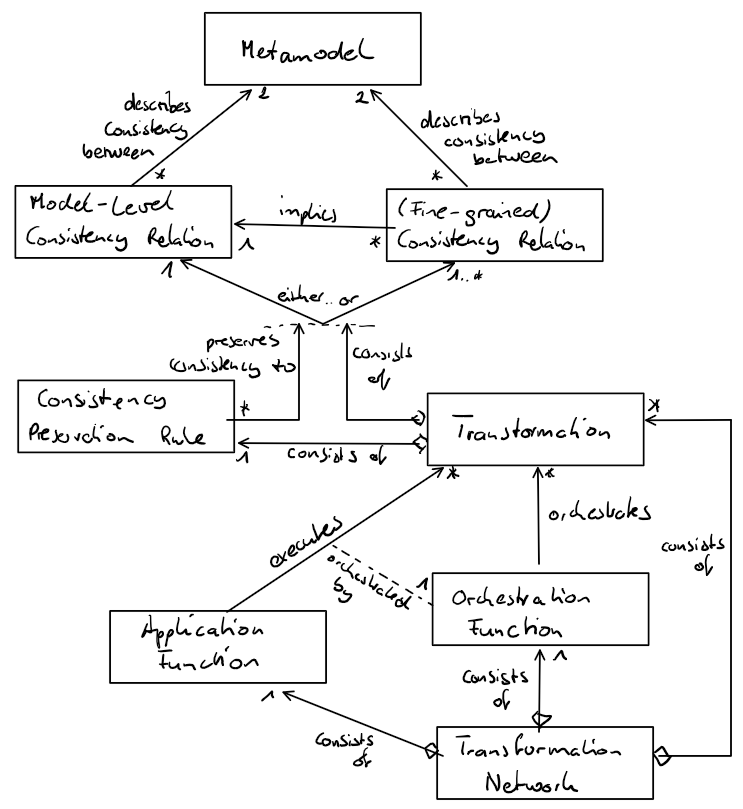
\includegraphics[width=0.85\textwidth]{figures/correctness/notion/conceptual_model.png}
    \caption[Conceptual model for transformation networks]{A conceptual model for the terms and artifacts introduced for transformation networks and their relations. Adapted from \owncite{klare2020Vitruv-JSS}.}
    \label{fig:correctness:conceptual_model}
\end{figure}

\mnote{Insight}
In this chapter, we have discussed notions of correctness for transformation networks and the artifacts it consist of, and we have precisely defined that notion that is relevant for the context of this thesis.
We give an overview of the introduced concepts and their relations in the conceptual model depicted in \autoref{fig:correctness:conceptual_model}.
In summary, we provided the following insight in this chapter.

\begin{insight}[Correctness Notion]
    A reasonable notion of correctness for networks of modular, independently developed transformations consists of correctness of the single transformations, which need to be synchronizing, and correctness of the application function that determines an execution order of the transformations.
    An application function may not be able to return a result due to different reasons, such as transformations not being applicable to specific changes, the absence of an execution order of the transformations that leads to consistent models, or the inability to find such an order.
    Thus, in comparison to correctness, the degree of conservativeness is the more important property of an application function, which indicates how often the function does not deliver a result although there is an order of transformations that would restore consistency.
    Additionally, although theoretically not relevant for correctness, the relations defining when models are considered consistent have to fulfill some notion of compatibility to be useful, as they can otherwise prevent transformations from finding consistent models.
    %Finally, we found that we can define a more fine-grained notion of consistency that is aligned with practical representations of consistency in transformation languages.
\end{insight}

\mnote{Achieving correct transformation networks}
In the following chapters, we will thus define a notion of compatibility for consistency relations, discuss how correctness of the individual synchronizing transformations for achieving local consistency can be achieved and finally how a correct and appropriate application function to perform the orchestration for achieving global consistency can be defined.
In summary, these following contributions together will allow to develop what we defined as a \emph{correct} transformation network.

\begin{figure}
    \centering
    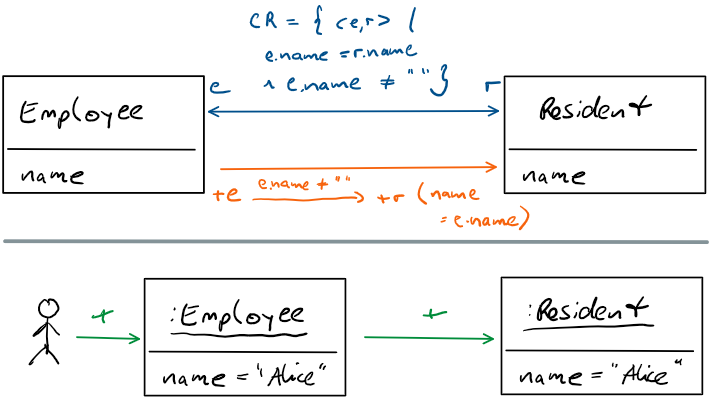
\includegraphics[width=0.8\textwidth]{figures/correctness/notion/visualization_example.png}
    \caption[Example for concept visualizations]{Example for visualization of consistency relations, consistency preservation rules and their execution.}
    \label{fig:correctness:visualization_example}
\end{figure}

For visualizing examples of consistency relations, consistency preservation rules and their execution throughout the next chapters, we use a notation according to the example depicted in \autoref{fig:correctness:visualization_example}.
We visualize consistency relations in blue with a definition of the conditions for consistency relation pairs forming that relation.
In the example, the consistency relation contains all pairs of employees and residents having the same name, expect for those with an empty name.
We depict consistency preservation rules in orange and denote which changes it produces because of which input change.
In the example, we denote that the addition of an employee ($+e$) leads to the addition of a resident with the same name, specified by the according property assignment $r(\mathvariable{name} = \mathvariable{e.name})$.
In addition, we annotate conditions to the consistency preservation rules, such as $\mathvariable{e.name} \neq \enquote{}$ in the example, which restricts the resident creation to the case in which the employee has a non-empty name.
We usually specify only parts of a consistency preservation rule, e.g., in the example we only specify the behavior for the case of adding an element but not of modifying or removing it.
Finally, we denote the execution of any changes, including consistency preservation rules, in green.
In the example, we visualize the addition of an employee by a user, denoted with a $+$, which leads to the addition of a resident, for example, because of the execution of the above introduced consistency preservation rule.


% \section{Summary}

% Central Insights:
% \begin{itemize}
%     \item In networks, we need compatible consistency relations -> first RQ
%     \item In networks, we need synchronizing rather than bidirectional transformations -> second RQ
%     \item In networks, we need orchestration functions -> third RQ
%     \item Correctness is not the problem, optimality is the problem
%     \item We can only check dynamically whether a consistent state was reached due to Halting Problem. We cannot guarantee to always find a consistent state
% \end{itemize}